%%%%%%%%%%%%%%%%%%%%%%%%
%
% $Autor: Sadegh Naderi $
% $Datum: 2023-11-24  $
% $Short Description: Overview of the KDD (Knowledge Discovery in Databases) Process chapter focusing on its role in handling large datasets, challenges in data mining, and its application to speech recognition with the Arduino Nano 33 BLE Sense $
% $Directory: ML23-01-Keyword-Spotting-with-an-Arduino-Nano-33-BLE-Sense/report/Contents/en/KDDIntroduction.tex $
% $Version: 2 $
% $Review by:Achal Shakywar $
% $Review date:16.12.2023$
%
%%%%%%%%%%%%%%%%%%%%%%%%

\chapter{\ac{kdd} Process}


\section{Introduction}

\ac{kdd} plays a pivotal role in helping organizations navigate the overwhelming volumes of data generated in today's information-driven world \cite{Fayyad:1996}. This process involves transforming raw data into actionable knowledge, uncovering hidden patterns, and providing valuable insights for decision-making. As we delve into the intricacies of the KDD framework, it becomes evident that this multidisciplinary approach has transformative potential across diverse sectors. 

This chapter aims to provide an understanding of the KDD process, shedding light on its  challenges, and the critical role it plays in harnessing the power of data to inform strategic and informed decision-making.


\section{Impracticality of Manual Data Analysis}

Traditional manual methods of data analysis and interpretation are becoming impractical as data volumes grow exponentially. With databases containing billions of records and numerous fields, human capacities are surpassed. Health-care specialists analyzing trends and planetary geologists cataloging geologic objects are few of the examples \cite{Fayyad:1996}. The need for automation in knowledge extraction from large databases becomes evident.


\section{The KDD Process Framework}

The KDD process, as depicted in the Figure \ref{fig:KDDProcess}, begins with a comprehensive understanding of the problem domain. This initiates two main phases: "Deployment" and "Development."

\begin{figure}[h!]
	\centering
	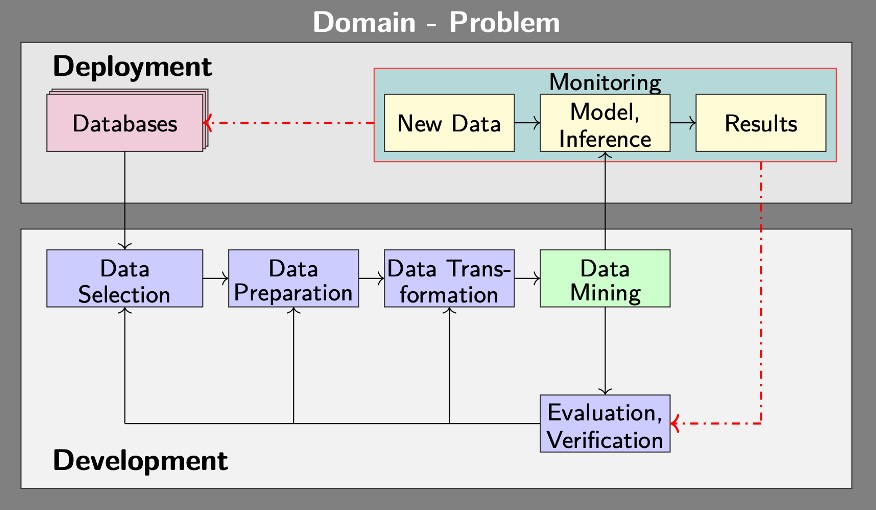
\includegraphics[width=0.8\textwidth]{Images/KDDProcess/KDDProcess}
	\caption{KDD Process Workflow \cite{Wings:2023}.} \label{fig:KDDProcess}
\end{figure}

In the "Deployment" phase, databases serve as the repository for relevant data. The arrow from "Databases" to "Data Selection" signifies the crucial step of selecting relevant data for analysis. 
at the same time, the "Monitoring" step oversees the ongoing processes, including the monitoring of new data, model inference, and results. This cyclic monitoring ensures adaptability to changing data conditions.

In the "Development" phase, a sequence of activities unfolds, starting with "Data Selection," followed by "Data Preparation," "Data Transformation," and ultimately "Data Mining." The arrows connecting these stages denote the sequential progression of operations.

From the "Data Mining" stage, two arrows extend: one leading to "Model Inference" and another to "Evaluation (Verification)." "Model Inference" involves deriving models from the mined data, while "Evaluation" assesses the performance and validity of these models.

The cyclical nature of the KDD process is highlighted through three feedback arrows from "Evaluation (Verification)" back to the initial stages of "Data Selection," "Data Preparation," and "Data Transformation." This iterative loop emphasizes continuous refinement based on the evaluation outcomes, fostering an adaptive and improving analytical process.

The "Monitoring" step contributes to the iterative nature of the process by providing feedback to "Databases," ensuring that the ongoing monitoring influences the selection of data from databases. Additionally, the "Results" step influences "Evaluation (Verification)," reinforcing the importance of the outcomes in guiding further verification or refinement.


\section{Challenges in Data Mining}

Data mining faces challenges such as impracticality due to massive datasets and high dimensionality, user interaction, overfitting, missing data, and the need for understandable patterns \cite{Fayyad:1996}. Integrating domain knowledge and addressing issues related to changing data, data types, and multimedia content are of high importance. 


\section{Why KDD Process for Speech Recognition?}

The Knowledge Discovery in Databases (KDD) process plays a crucial role in keyword spotting for several reasons:



\begin{enumerate}
	\item \textbf{Data Abundance and Complexity:} The Arduino Nano 33 BLE Sense is likely to generate substantial amounts of sensor data. KDD provides a systematic approach to handling large volumes of diverse data, allowing efficient extraction of meaningful patterns and insights.
	
	\item \textbf{Feature Extraction and Selection:} Keyword spotting involves identifying specific patterns within the collected data. KDD assists in selecting and extracting relevant features from raw sensor data, optimizing the data for accurate keyword detection.
	
	\item \textbf{Adaptability to Changing Conditions:} The iterative nature of KDD, with feedback loops and continuous monitoring, is valuable for adapting the model to changing conditions. This ensures sustained performance over time.
	
	\item \textbf{Evaluation and Verification:} KDD emphasizes evaluating models to ensure their effectiveness. In keyword spotting, it ensures the model performs accurately, providing insights for improvement and fine-tuning.
	
	\item \textbf{Interpretability and Understandability:} KDD places emphasis on finding patterns that are not only accurate but also understandable. This is crucial in keyword spotting for developing transparent and interpretable models.
	
\end{enumerate}


\section{Conclusion}

Despite its rapid growth, the field of KDD is still in its infancy \cite{Fayyad:1996}. A balanced approach is needed to be taken, ensuring that the potential contributions of KDD are not overstated, and users understand both the capabilities and limitations of KDD tools. While challenges persist, the societal and economic needs for managing and analyzing vast amounts of data continue to drive the growth of KDD, making it a field with significant potential for future developments.

